\documentclass[aspectratio=169,11pt]{beamer}

\usepackage[T1]{fontenc}
\usepackage{lmodern}
\usepackage{booktabs}
\usepackage{algorithm2e}
% Shared TikZ styles, colours and the running example.
% Used by both slides/slides.tex and notes/lecture.tex.
%
% Running example (X = {a,...,e}, Y = {1,...,5}):
%   edges  a1 a3 | b2 b5 | c4 c5 | d1 d2 | e1
%   Phase 1: shortest aug. path length 1  -> a1, b2, c4
%   Phase 2: shortest aug. path length 3  -> d1 a3
%   Phase 3: shortest aug. path length 5  -> e1 d2 b5   (perfect matching)

\usepackage{amsmath,amssymb,mathtools}
\usepackage{tikz}
\usetikzlibrary{arrows.meta,positioning,calc,fit,backgrounds,decorations.pathreplacing,shapes.geometric}

\definecolor{hkblue}{HTML}{2F5D9B}
\definecolor{hkorange}{HTML}{D1793A}
\definecolor{hkred}{HTML}{C0392B}
\definecolor{hkgreen}{HTML}{2E8B57}
\definecolor{hkgrey}{HTML}{6B6B6B}

\newcommand{\symdiff}{\oplus}
\newcommand{\M}{M}
\newcommand{\bigO}[1]{O\!\left(#1\right)}

\tikzset{
  boy/.style={circle, draw=hkblue!80, fill=hkblue!16, minimum size=6.6mm,
              inner sep=0pt, font=\footnotesize, thick},
  girl/.style={circle, draw=hkorange!90, fill=hkorange!22, minimum size=6.6mm,
               inner sep=0pt, font=\footnotesize, thick},
  freev/.style={draw=hkgreen, line width=1.3pt},   % ring that marks a free vertex
  unm/.style={line width=0.6pt, draw=black!35},          % unmatched edge
  mat/.style={line width=1.9pt, draw=black!80},          % matching edge
  aug/.style={line width=2.2pt, draw=hkred},             % edge on augmenting path
  Medge/.style={line width=1.9pt, draw=hkblue},
  Nedge/.style={line width=1.9pt, draw=hkorange, dashed},
  layerlab/.style={font=\footnotesize\bfseries, text=hkblue!85!black},
}

% ---- the running example --------------------------------------------------
% left column top->bottom: a e d b c ; right column: 3 1 2 5 4   (planar drawing)
\newcommand{\exnodes}{%
  \node[boy]  (xa) at (0, 2.2) {$a$};
  \node[boy]  (xe) at (0, 1.1) {$e$};
  \node[boy]  (xd) at (0, 0.0) {$d$};
  \node[boy]  (xb) at (0,-1.1) {$b$};
  \node[boy]  (xc) at (0,-2.2) {$c$};
  \node[girl] (y3) at (2.8, 2.2) {$3$};
  \node[girl] (y1) at (2.8, 1.1) {$1$};
  \node[girl] (y2) at (2.8, 0.0) {$2$};
  \node[girl] (y5) at (2.8,-1.1) {$5$};
  \node[girl] (y4) at (2.8,-2.2) {$4$};
}
\newcommand{\exedges}{%
  \draw[unm] (xa)--(y1); \draw[unm] (xa)--(y3);
  \draw[unm] (xb)--(y2); \draw[unm] (xb)--(y5);
  \draw[unm] (xc)--(y4); \draw[unm] (xc)--(y5);
  \draw[unm] (xd)--(y1); \draw[unm] (xd)--(y2);
  \draw[unm] (xe)--(y1);
}
% highlight a vertex as free
\newcommand{\freering}[1]{\draw[freev] (#1) circle (4.4mm);}


% ------------------------------------------------------------------ theme
\usetheme{default}
\setbeamercolor{structure}{fg=hkblue}
\setbeamercolor{frametitle}{fg=hkblue}
\setbeamercolor{block title}{bg=hkblue!14,fg=hkblue!85!black}
\setbeamercolor{block body}{bg=hkblue!5}
\setbeamercolor{block title alerted}{bg=hkred!14,fg=hkred!90!black}
\setbeamercolor{block body alerted}{bg=hkred!5}
\setbeamercolor{block title example}{bg=hkgreen!16,fg=hkgreen!55!black}
\setbeamercolor{block body example}{bg=hkgreen!6}
\setbeamercolor{alerted text}{fg=hkred}
\setbeamerfont{frametitle}{size=\Large,series=\bfseries}
\setbeamerfont{block title}{size=\normalsize,series=\bfseries}
\setbeamertemplate{navigation symbols}{}
\setbeamertemplate{blocks}[rounded][shadow=false]
\setbeamertemplate{itemize items}[circle]

\setbeamertemplate{frametitle}{%
  \vskip1.2ex
  \hspace*{0.2cm}\usebeamercolor[fg]{frametitle}\usebeamerfont{frametitle}\insertframetitle\par
  \vskip-0.4ex
  \hspace*{0.2cm}{\color{hkblue!55}\rule{\dimexpr\paperwidth-0.6cm\relax}{0.6pt}}%
}

\newcommand{\curspk}{Viswanadha Bhanu Sriharsha}
\newif\ifbackup \newcommand{\mainframes}{18}  % number of frames before \appendix
\newcommand{\curpart}{Problem}
\setbeamertemplate{footline}{%
  \leavevmode\hbox to\paperwidth{%
    \hspace{0.3cm}{\footnotesize\color{hkgrey}Hopcroft--Karp (1973) \textperiodcentered\ \curpart}%
    \hfill{\footnotesize\color{hkgrey}\curspk\quad \insertframenumber\ifbackup\else\,/\,\mainframes\fi}\hspace{0.3cm}}%
  \vskip1.2ex}

\title{The Hopcroft--Karp Algorithm}
\author{Viswanadha Bhanu Sriharsha \and Aman Pathak}
\date{CS-G526 \textperiodcentered\ November 2026}

\DontPrintSemicolon
\SetAlgoLined
\SetKwComment{Comment}{// }{}

% "In plain words" box
\newenvironment{plain}[1][In plain words]{\begin{exampleblock}{#1}}{\end{exampleblock}}

% arrows for the directed layered graph
\tikzset{darr/.style={-{Stealth[length=2mm]},line width=0.7pt,draw=black!45},
         dmat/.style={-{Stealth[length=2.2mm]},line width=1.8pt,draw=black!80},
         dred/.style={-{Stealth[length=2.2mm]},line width=2.2pt,draw=hkred}}

% layered graph (paper's direction: arrows point from s towards t, i.e. to the left)
% layer i drawn at x = 2.2*i ; M = {a1,b2,c4}
\newcommand{\layerNodes}{%
  \node[boy]  (Ld) at (0,0.8)  {$d$};
  \node[boy]  (Le) at (0,-0.8) {$e$};
  \node[girl] (L1) at (2.2,0.8)  {$1$};
  \node[girl] (L2) at (2.2,-0.8) {$2$};
  \node[boy]  (La) at (4.4,0.8)  {$a$};
  \node[boy]  (Lb) at (4.4,-0.8) {$b$};
  \node[girl] (L3) at (6.6,0.8)  {$3$};
  \node[girl] (L5) at (6.6,-0.8) {$5$};
}
\newcommand{\layerLabels}{%
  \node[layerlab] at (0,1.7)   {$L_0$};
  \node[layerlab] at (2.2,1.7) {$L_1$};
  \node[layerlab] at (4.4,1.7) {$L_2$};
  \node[layerlab] at (6.6,1.7) {$L_3$};
}


% chalk-and-board cue: small tag in the top-right corner of a frame
\newcommand{\board}[1]{\begin{tikzpicture}[remember picture,overlay]
  \node[anchor=north east,fill=hkorange!18,draw=hkorange,rounded corners=2pt,font=\scriptsize\bfseries,
        text=hkorange!55!black,inner sep=3pt] at ([xshift=-0.3cm,yshift=-0.25cm]current page.north east){BOARD: #1};
\end{tikzpicture}}

\begin{document}

% ======================================================================
% 1  TITLE
% ======================================================================
\begin{frame}[plain]
\begin{tikzpicture}[remember picture,overlay]
  \fill[hkblue!6] (current page.south west) rectangle (current page.north east);
  \fill[hkblue] (current page.north west) rectangle ([yshift=-3mm]current page.north east);
\end{tikzpicture}
\vspace{0.5cm}
\begin{columns}[c,onlytextwidth]
\column{0.64\textwidth}
  {\color{hkblue}\fontsize{26}{30}\selectfont\bfseries The Hopcroft--Karp\\[1mm] Algorithm\par}
  \vspace{4mm}
  {\Large\color{black!70} Maximum matchings in bipartite graphs\\ in $O\big((m+n)\sqrt n\,\big)$ time\par}
  \vspace{9mm}
  {\large \textcolor{hkblue}{Viswanadha Bhanu Sriharsha} \ (2026H1030024G)\par}
  {\large \textcolor{hkorange}{Aman Pathak} \ (2026PHXP0018G)\par}
  \vspace{1mm}
  {\normalsize CS-G526 \textperiodcentered\ November 2026\par}
  \vspace{8mm}
  {\footnotesize\color{hkgrey}J.\,E.\ Hopcroft and R.\,M.\ Karp,
   \emph{An $n^{5/2}$ algorithm for maximum matchings in bipartite graphs},
   SIAM J.\ Comput.\ 2(4):225--231, 1973.\par}
\column{0.34\textwidth}
\centering
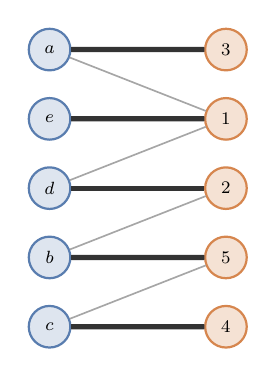
\begin{tikzpicture}[scale=0.8,transform shape]
  \exnodes \exedges
  \draw[mat] (xa)--(y3); \draw[mat] (xb)--(y5); \draw[mat] (xc)--(y4);
  \draw[mat] (xd)--(y2); \draw[mat] (xe)--(y1);
\end{tikzpicture}
\end{columns}
\end{frame}

% ======================================================================
% 3  THE PROBLEM
% ======================================================================
\begin{frame}{The problem}
\begin{columns}[c]
\column{0.5\textwidth}
\centering
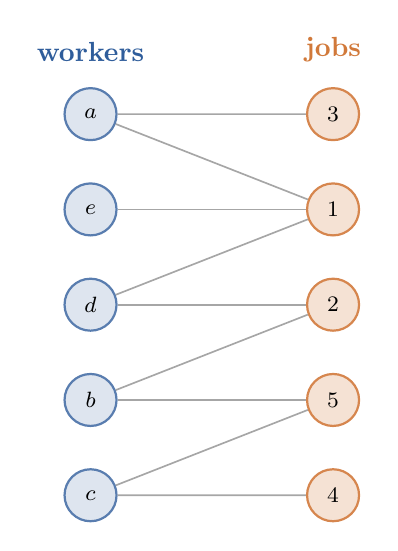
\begin{tikzpicture}[scale=1.1]
  \exnodes \exedges
  \node[above=2mm of xa, font=\normalsize\bfseries, text=hkblue] {workers};
  \node[above=2mm of y3, font=\normalsize\bfseries, text=hkorange] {jobs};
\end{tikzpicture}
\column{0.46\textwidth}
{\Large Five workers, five jobs.\par}\vspace{4mm}
{\Large Each worker takes one job.\\ Each job gets one worker.\par}\vspace{8mm}
{\Large\bfseries\color{hkred} How many jobs can we fill?\par}
\end{columns}
\end{frame}

% ======================================================================
% 4  DEFINITIONS, APPLICATIONS, PRIOR WORK
% ======================================================================
\begin{frame}{Three words}
\Large
\vspace{3mm}
\textbf{\color{hkblue}Matching}\quad a set of edges, no two share a vertex.\\[5mm]
\textbf{\color{hkblue}Free vertex}\quad no matching edge touches it.\\[5mm]
\textbf{\color{hkblue}Maximum}\quad no matching is bigger.\\[10mm]
{\color{hkgrey}Before 1973: $O(mn)$.}\quad {\color{hkred}\textbf{Today's goal: $O(m\sqrt n)$.}}
\end{frame}

% ======================================================================
% 5  GREEDY
% ======================================================================
\begin{frame}{First attempt: greedy}
\begin{columns}[c]
\column{0.46\textwidth}
\centering
\begin{tikzpicture}[scale=1.1]
  \exnodes \exedges
  \draw[mat] (xa)--(y1);
  \only<2->{\draw[mat] (xb)--(y2);}
  \only<3->{\draw[mat] (xc)--(y4);}
  \only<4->{\freering{xd}\freering{xe}\freering{y3}\freering{y5}}
\end{tikzpicture}
\column{0.5\textwidth}
\large
Grab an edge whenever both ends are free.\\[4mm]
\begin{itemize}\setlength\itemsep{4pt}
  \item<1-> $a\!-\!1$
  \item<2-> $b\!-\!2$
  \item<3-> $c\!-\!4$
  \item<4-> $d$ and $e$ are stuck.
\end{itemize}
\vspace{3mm}
\onslide<5->{{\Large\bfseries\color{hkred} Maximal, not maximum.}\\[1mm]
{\normalsize Five pairs are possible.}}
\end{columns}
\end{frame}

% ======================================================================
% 6  CHAIN REACTION
% ======================================================================
\renewcommand{\curpart}{II. Augmenting paths}
\begin{frame}{The repair}
\begin{columns}[c]
\column{0.46\textwidth}
\centering
\begin{tikzpicture}[scale=1.1]
  \exnodes \exedges
  \draw[mat] (xb)--(y2); \draw[mat] (xc)--(y4);
  \only<1-4>{\draw[mat] (xa)--(y1);}
  \only<5->{\draw[mat] (xa)--(y3); \draw[mat] (xd)--(y1);}
  \only<1>{\freering{xd}\freering{y3}}
  \only<2-4>{\draw[aug] (xd)--(y1); \freering{xd}\freering{y3}}
  \only<3-4>{\draw[aug] (xa)--(y1);}
  \only<4>{\draw[aug] (xa)--(y3);}
\end{tikzpicture}
\column{0.5\textwidth}
\large
\begin{enumerate}\setlength\itemsep{9pt}
  \item<1-> $d$ has no job.
  \item<2-> $d$ wants job 1.
  \item<3-> Job 1 is $a$'s.
  \item<4-> $a$ can take job 3.
  \item<5-> $d$ takes 1. \textbf{One more pair.}
\end{enumerate}
\end{columns}
\end{frame}

% ======================================================================
% 7  AUGMENTING PATH + LEMMA 1
% ======================================================================
\begin{frame}{Augmenting paths}
\board{flip a path, count edges}
\vspace{4mm}
\centering
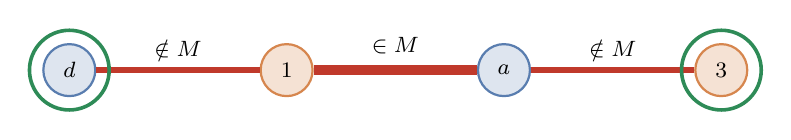
\begin{tikzpicture}[scale=1.15]
  \node[boy] (a) at (0,0) {$d$};  \node[girl] (b) at (2.4,0) {$1$};
  \node[boy] (c) at (4.8,0) {$a$}; \node[girl] (d) at (7.2,0) {$3$};
  \draw[aug] (a)--node[above,font=\footnotesize]{$\notin M$}(b);
  \draw[aug,line width=3.4pt] (b)--node[above=1pt,font=\footnotesize]{$\in M$}(c);
  \draw[aug] (c)--node[above,font=\footnotesize]{$\notin M$}(d);
  \freering{a}\freering{d}
\end{tikzpicture}\\[8mm]
{\Large Free end to free end, edges alternate.\par}\vspace{6mm}
{\Large\bfseries\color{hkred} Flip it: the matching grows by one.\par}\vspace{2mm}
{\normalsize\color{hkgrey} Lemma 1}
\end{frame}

% ======================================================================
% 9  CORROLLARY 1 + CLASSICAL ALGORITHM
% ======================================================================
\begin{frame}{Berge's theorem}
\board{proof of Theorem 1}
\vspace{2mm}
\begin{block}{Theorem 1}
A bigger matching $N$ gives at least $|N|-|M|$ disjoint augmenting paths for $M$.
\end{block}
\vspace{4mm}
\begin{center}
{\Large $M$ is maximum $\iff$ no augmenting path.}\\[1mm]
{\normalsize\color{hkgrey} Corollary 1 (Berge)}
\end{center}
\vspace{5mm}
{\large Repeat: find a path, flip it.\\[2mm]
At most $n/2$ flips, $O(m)$ per search:\quad {\Large\bfseries\color{hkred}$O(mn)$}.}
\end{frame}

% ======================================================================
% 10  THE PLAN: SHORTEST AUGMENTING PATHS AND THE SEQUENCE
% ======================================================================
\renewcommand{\curspk}{Aman Pathak}
\renewcommand{\curpart}{III. Shortest paths and phases}
\begin{frame}{Take many at once?}
\begin{columns}[c]
\column{0.5\textwidth}
\centering
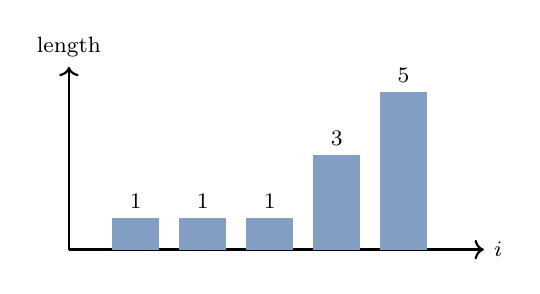
\begin{tikzpicture}[x=0.85cm,y=0.4cm]
  \draw[->,thick] (0,0)--(6.2,0) node[right,font=\footnotesize]{$i$};
  \draw[->,thick] (0,0)--(0,5.8) node[above,font=\footnotesize]{length};
  \foreach \i/\h in {1/1,2/1,3/1,4/3,5/5}{
    \fill[hkblue!60] (\i-0.35,0) rectangle (\i+0.35,\h);
    \node[font=\footnotesize,above] at (\i,\h) {$\h$};}
\end{tikzpicture}\\[1mm]
{\footnotesize our five paths: $a1,\,b2,\,c4,\,d1a3,\,e1d2b5$}
\column{0.46\textwidth}
{\Large Always flip a \emph{shortest} path.\par}\vspace{5mm}
\large
\begin{enumerate}\setlength\itemsep{6pt}
  \item Lengths never shrink.
  \item Same length: disjoint.
  \item Only $\sqrt n$ different lengths.
\end{enumerate}
\end{columns}
\end{frame}

% ======================================================================
% 11  THEOREM 2
% ======================================================================
\begin{frame}{Theorem 2}
\board{proof of Theorem 2}
\vspace{3mm}
\begin{block}{Theorem 2}
$P$ is a shortest augmenting path for $M$, and $P'$ is augmenting for $M\oplus P$. Then $|P'|\ge|P|$.
\end{block}
\vspace{8mm}
\begin{center}
{\Large Flip a shortest path:\\[2mm] the other paths get no closer.\par}
\end{center}
\end{frame}

% ======================================================================
% 12  COROLLARIES 3 AND 4
% ======================================================================
\begin{frame}{Corollaries 3 and 4}
\begin{columns}[c]
\column{0.5\textwidth}
\begin{block}{Corollary 3}
Lengths never decrease.
\end{block}
\begin{block}{Corollary 4}
Same length $\Rightarrow$ vertex-disjoint.
\end{block}
\column{0.46\textwidth}
\centering
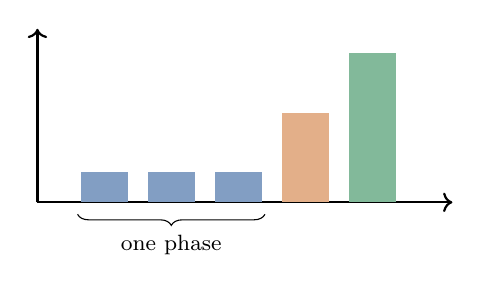
\begin{tikzpicture}[x=0.85cm,y=0.38cm]
  \draw[->,thick] (0,0)--(6.2,0);
  \draw[->,thick] (0,0)--(0,5.8);
  \foreach \i/\h/\c in {1/1/hkblue,2/1/hkblue,3/1/hkblue,4/3/hkorange,5/5/hkgreen}{
    \fill[\c!60] (\i-0.35,0) rectangle (\i+0.35,\h);}
  \draw[decorate,decoration={brace,mirror,amplitude=4pt}] (0.6,-0.4)--(3.4,-0.4) node[midway,below=4pt,font=\footnotesize]{one phase};
\end{tikzpicture}
\end{columns}
\vspace{6mm}
\centering{\Large A block of equal length can be found \textbf{at once}.\par}
\end{frame}

% ======================================================================
% 13  ALGORITHM A
% ======================================================================
\begin{frame}{Algorithm A}
\Large
\begin{block}{Algorithm A}
\textbf{0.} Start with $M=\emptyset$.\\[2pt]
\textbf{1.} Find a \emph{maximal} set of disjoint shortest augmenting paths.\\[2pt]
\textbf{2.} Flip them all. Repeat.
\end{block}
\vspace{6mm}
\normalsize
\begin{center}
{\large Each phase makes the shortest length \textbf{grow}.}
\end{center}
\end{frame}

% ======================================================================
% 15  THEOREM 3 / COR 5
% ======================================================================
\begin{frame}{How many phases?}
\board{the split at $s-\sqrt s$}
\vspace{2mm}
\begin{block}{Theorem 3}
At most $2\lfloor\sqrt s\rfloor+2$ phases, where $s$ is the size of a maximum matching.
\end{block}
\vspace{8mm}
\centering
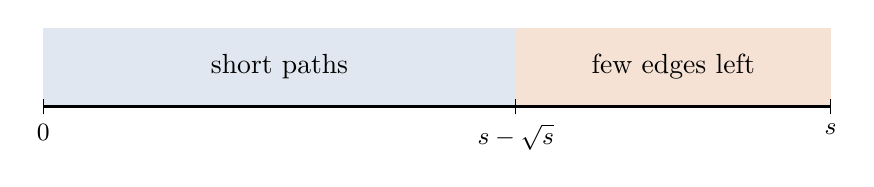
\begin{tikzpicture}[x=1.0cm,y=1cm]
  \fill[hkblue!15] (0,0) rectangle (6,1);
  \fill[hkorange!22] (6,0) rectangle (10,1);
  \draw[thick] (0,0)--(10,0);
  \foreach \x/\t in {0/{0},6/{$s-\sqrt s$},10/{$s$}} {\draw (\x,-0.1)--(\x,0.1); \node[font=\small,below] at (\x,-0.1) {\t};}
  \node[font=\normalsize] at (3,0.5) {short paths};
  \node[font=\normalsize] at (8,0.5) {few edges left};
\end{tikzpicture}
\end{frame}

% ======================================================================
% 16  BIPARTITE CASE: ORIENT EDGES
% ======================================================================
\renewcommand{\curpart}{IV. One phase in $O(m+n)$}
\begin{frame}{One phase: orient the edges}
\begin{columns}[c]
\column{0.5\textwidth}
\centering
\begin{tikzpicture}[scale=1.1]
  \exnodes
  \only<1>{\exedges \draw[mat] (xa)--(y1); \draw[mat] (xb)--(y2); \draw[mat] (xc)--(y4);}
  \only<2->{%
    \draw[dmat] (xa)--(y1); \draw[dmat] (xb)--(y2); \draw[dmat] (xc)--(y4);
    \draw[darr] (y3)--(xa); \draw[darr] (y5)--(xb); \draw[darr] (y5)--(xc);
    \draw[darr] (y1)--(xd); \draw[darr] (y2)--(xd); \draw[darr] (y1)--(xe);}
  \only<3->{\draw[dred] (y3)--(xa); \draw[dred] (xa)--(y1); \draw[dred] (y1)--(xd);}
  \freering{xd}\freering{xe}\freering{y3}\freering{y5}
\end{tikzpicture}
\column{0.46\textwidth}
\large
\begin{itemize}\setlength\itemsep{8pt}
  \item<2-> Not in $M$: girl $\to$ boy.
  \item<2-> In $M$: boy $\to$ girl.
  \item<3-> An augmenting path is now a \textbf{directed path}.
\end{itemize}
\end{columns}
\end{frame}

% ======================================================================
% 17  LAYERED GRAPH
% ======================================================================
\begin{frame}{The layered graph}
\begin{columns}[c]
\column{0.68\textwidth}
\centering
\begin{tikzpicture}[scale=0.85]
  \layerNodes
  \only<1->{\node[layerlab] at (0,1.7) {$L_0$};}
  \only<2->{\node[layerlab] at (2.2,1.7) {$L_1$};}
  \only<3->{\node[layerlab] at (4.4,1.7) {$L_2$};}
  \only<4->{\node[layerlab] at (6.6,1.7) {$L_3$};}
  \freering{Ld}\freering{Le}\freering{L3}\freering{L5}
  \only<2->{\draw[darr] (L1)--(Ld); \draw[darr] (L1)--(Le); \draw[darr] (L2)--(Ld);}
  \only<3->{\draw[dmat] (La)--(L1); \draw[dmat] (Lb)--(L2);}
  \only<4->{\draw[darr] (L3)--(La); \draw[darr] (L5)--(Lb);}
  \only<5->{\node[draw,rounded corners,fill=hkgrey!15,inner sep=3pt,font=\footnotesize] (S) at (8.7,0) {$s$};
            \node[draw,rounded corners,fill=hkgrey!15,inner sep=3pt,font=\footnotesize] (T) at (-1.9,0) {$t$};
            \draw[darr] (S)--(L3); \draw[darr] (S)--(L5); \draw[darr] (Ld)--(T); \draw[darr] (Le)--(T);}
\end{tikzpicture}
\column{0.28\textwidth}
\large
\begin{itemize}\setlength\itemsep{8pt}
  \item<1-> Start at the free boys.
  \item<2-> Walk back, level by level.
  \item<4-> Stop at a free girl.
  \item<5-> Add $s$ and $t$.
\end{itemize}
\end{columns}
\end{frame}

% ======================================================================
% 18  ALGORITHM B
% ======================================================================
\begin{frame}{Algorithm B}
\centering
\begin{minipage}{0.7\textwidth}
\begin{algorithm}[H]
\normalsize
\SetAlgoLined
\SetAlgoNoEnd
\SetInd{0.6em}{0.9em}
PUSH $s$\;
\While{STACK $\neq\emptyset$}{
  \While{LIST(TOP) $\neq\emptyset$}{
    FIRST $\gets$ first element of LIST(TOP); \textbf{DELETE} it\;
    \If{FIRST $\notin B$}{
      PUSH FIRST\;
      \lIf{TOP $=t$}{PRINT path; PUSH $s$}\lElse{$B\gets B\cup\{\text{TOP}\}$}
    }
  }
  POP\;
}
\end{algorithm}
\end{minipage}\\[5mm]
{\Large Every edge we look at is \textbf{deleted}.\par}
\end{frame}

% ======================================================================
% 19  ALGORITHM B WALKTHROUGH
% ======================================================================
\begin{frame}{Algorithm B on the example}
\centering
\begin{tikzpicture}[scale=0.95]
  \layerNodes
  \node[draw,rounded corners,fill=hkgrey!15,inner sep=3pt,font=\footnotesize] (S) at (8.7,0) {$s$};
  \node[draw,rounded corners,fill=hkgrey!15,inner sep=3pt,font=\footnotesize] (T) at (-1.9,0) {$t$};
  \draw[darr] (L1)--(Ld); \draw[darr] (L1)--(Le); \draw[darr] (L2)--(Ld);
  \draw[dmat] (La)--(L1); \draw[dmat] (Lb)--(L2);
  \draw[darr] (L3)--(La); \draw[darr] (L5)--(Lb);
  \draw[darr] (S)--(L3); \draw[darr] (S)--(L5); \draw[darr] (Ld)--(T); \draw[darr] (Le)--(T);
  \only<1>{\draw[dred] (S)--(L3);}
  \only<2>{\draw[dred] (S)--(L3); \draw[dred] (L3)--(La); \draw[dred] (La)--(L1);}
  \only<3>{\draw[dred] (S)--(L3); \draw[dred] (L3)--(La); \draw[dred] (La)--(L1); \draw[dred] (L1)--(Ld); \draw[dred] (Ld)--(T);}
  \only<4->{\draw[dred] (S)--(L3); \draw[dred] (L3)--(La); \draw[dred] (La)--(L1); \draw[dred] (L1)--(Ld); \draw[dred] (Ld)--(T);}
  \only<4->{\draw[hkorange,line width=2.2pt,-{Stealth[length=2.2mm]}] (S)--(L5); \draw[hkorange,line width=2.2pt,-{Stealth[length=2.2mm]}] (L5)--(Lb); \draw[hkorange,line width=2.2pt,-{Stealth[length=2.2mm]}] (Lb)--(L2);}
  \only<5>{\draw[hkred,thick] ($(L2)+(-0.3,-0.3)$)--($(L2)+(0.3,0.3)$) ($(L2)+(-0.3,0.3)$)--($(L2)+(0.3,-0.3)$);}
\end{tikzpicture}\\[5mm]
\large
\only<1>{$s,\,3$}%
\only<2>{$s,\,3,\,a,\,1$}%
\only<3>{$s,3,a,1,d,t$ \;$\Rightarrow$\; \textbf{path found:} $d1a3$}%
\only<4>{$s,\,5,\,b,\,2$\quad $2$ only leads to $d$, already used.}%
\only<5>{Dead end. Stack empty: \textbf{stop}.}
\end{frame}

% ======================================================================
% 22  PUTTING IT TOGETHER
% ======================================================================
\begin{frame}{The bound}
\vspace{4mm}
\begin{block}{Running time}
\[
  O(\sqrt n)\ \text{phases}\ \times\ O(m+n)\ \text{per phase}\ =\ O\big((m+n)\sqrt n\big)
\]
\end{block}
\vspace{8mm}
\centering
{\Huge\bfseries\color{hkred} $O(m\sqrt n)$}\\[4mm]
{\large instead of $O(mn)$}
\end{frame}

% ======================================================================
% 23  BEYOND + SUMMARY
% ======================================================================
\begin{frame}{Summary}
\Large
\begin{enumerate}\setlength\itemsep{8pt}
  \item Augmenting paths repair a matching.
  \item None left $\Leftrightarrow$ maximum (Berge).
  \item Flip a batch of shortest paths per phase.
  \item Only $O(\sqrt n)$ phases.
  \item Each phase: BFS and DFS, $O(m+n)$.
\end{enumerate}
\vspace{6mm}
\centering{\Huge\color{hkblue}\textbf{Questions?}}
\end{frame}

% ======================================================================
\appendix
\renewcommand{\curpart}{Backup}
\renewcommand{\curspk}{}\backuptrue

% ======================================================================
% 8  THEOREM 1
% ======================================================================
\begin{frame}{Theorem 1: comparing two matchings}
\begin{block}{Theorem 1}
If $M,N$ are matchings with $|M|=r<|N|=s$, then $M\oplus N$ contains at least $s-r$ \textbf{vertex-disjoint augmenting paths} relative to $M$.
\end{block}
\vspace{-1mm}
\begin{columns}[T]
\column{0.55\textwidth}
\footnotesize
\textbf{Proof.} Look at $H=(V,M\oplus N)$: only edges in exactly one of the two.
\begin{itemize}\setlength\itemsep{2pt}
  \item Each vertex has $\le1$ edge of $M$ and $\le1$ of $N$, so degree $\le2$: components are \textbf{isolated vertices, even cycles, or paths}, alternating $M,N$.
  \item $\delta(C)=|C\cap N|-|C\cap M|\in\{-1,0,1\}$, and $\delta=+1$ iff $C$ is augmenting for $M$.
  \item $\sum_C\delta(C)=|N|-|M|=s-r$, so at least $s-r$ components have $\delta=+1$. \hfill$\square$
\end{itemize}
\column{0.43\textwidth}
\centering
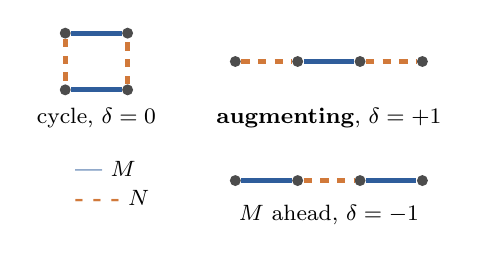
\begin{tikzpicture}[scale=0.72,v/.style={circle,fill=black!70,inner sep=1.4pt}]
  \node[v](c1) at (0,0){}; \node[v](c2) at (1.1,0){}; \node[v](c3) at (1.1,1){}; \node[v](c4) at (0,1){};
  \draw[Medge](c1)--(c2); \draw[Nedge](c2)--(c3); \draw[Medge](c3)--(c4); \draw[Nedge](c4)--(c1);
  \node[font=\footnotesize] at (0.55,-0.5) {cycle, $\delta=0$};
  \node[v](p1) at (3,0.5){}; \node[v](p2) at (4.1,0.5){}; \node[v](p3) at (5.2,0.5){}; \node[v](p4) at (6.3,0.5){};
  \draw[Nedge](p1)--(p2); \draw[Medge](p2)--(p3); \draw[Nedge](p3)--(p4);
  \node[font=\footnotesize,align=center] at (4.65,-0.5) {\textbf{augmenting}, $\delta=+1$};
  \node[v](q1) at (3,-1.6){}; \node[v](q2) at (4.1,-1.6){}; \node[v](q3) at (5.2,-1.6){}; \node[v](q4) at (6.3,-1.6){};
  \draw[Medge](q1)--(q2); \draw[Nedge](q2)--(q3); \draw[Medge](q3)--(q4);
  \node[font=\footnotesize] at (4.65,-2.2) {$M$ ahead, $\delta=-1$};
  \node[font=\footnotesize,anchor=west] at (0,-1.4) {\textcolor{hkblue}{\textbf{---}} $M$};
  \node[font=\footnotesize,anchor=west] at (0,-1.9) {\textcolor{hkorange}{\textbf{- - -}} $N$};
\end{tikzpicture}
\end{columns}
\vspace{1mm}
{\small\textbf{In plain words:} a better matching must differ from ours by $N$-heavy chains, and those chains are exactly the repairs we know how to make.}
\end{frame}

% ======================================================================
% 14  COROLLARY 2
% ======================================================================
\begin{frame}{Corollary 2: far from optimal means a short path exists}
\begin{block}{Corollary 2}
If $|M|=r$ and a maximum matching has size $s>r$, then there is an augmenting path of length at most $2\lfloor r/(s-r)\rfloor+1$.
\end{block}
\begin{columns}[T]
\column{0.54\textwidth}
\small\textbf{Proof.}
\begin{enumerate}\setlength\itemsep{2pt}
  \item Let $N$ be maximum. Theorem 1: $M\oplus N$ has $s-r$ vertex-disjoint augmenting paths for $M$.
  \item Together they contain at most $|M|=r$ edges of $M$ (disjoint!).
  \item So one has at most $\lfloor r/(s-r)\rfloor$ edges of $M$.
  \item An augmenting path with $k$ edges of $M$ has $2k+1$ edges. \hfill$\square$
\end{enumerate}
\column{0.44\textwidth}
\small
\begin{plain}
Many improvements are still missing ($s-r$ large), and they must share the little matching we have. So some improvement is cheap. Only when $M$ is \emph{nearly} maximum can every augmenting path be long.
\end{plain}
{\footnotesize Example: $r=3$, $s=5$: length $\le3$; phase 2 has length 3.}
\end{columns}
\end{frame}

% ======================================================================
% 20  CORRECTNESS + COMPLEXITY OF ALGORITHM B
% ======================================================================
\begin{frame}{Why Algorithm B works, and what it costs}
\begin{columns}[T]
\column{0.54\textwidth}
\small
\textbf{Invariant (paper).} Each time the algorithm is at the line ``PUSH FIRST'', for every vertex $u\ne s,t$:
\begin{center}\small
\begin{tabular}{@{}cp{5.6cm}@{}}
\toprule
(a) & $u\in B$, on a path already printed\\
(b) & $u\in B$, on the stack\\
(c) & $u\in B$, on \emph{no} $s$--$t$ path disjoint from the printed ones\\
(d) & $u\notin B$: untouched, all its edges present\\
\bottomrule
\end{tabular}
\end{center}
And the stack always holds a path from $s$ to TOP.
\column{0.46\textwidth}
\begin{plain}[So]
When the stack becomes empty, no $s$--$t$ path avoids the printed ones: the set is \textbf{maximal}.
\end{plain}
\vspace{2mm}
\begin{alertblock}{Cost}
Every pass of an inner loop \textbf{deletes an edge} or \textbf{pops a vertex}, and neither happens twice. Hence $O(m+n)$ per phase.
\end{alertblock}
\end{columns}
{\small\textbf{Building $\widetilde G$ is also linear:} one BFS, each vertex enters a level once and each edge is looked at once: $O(m+n)$.}
\end{frame}

% ======================================================================
% 21  WHOLE RUN
% ======================================================================
\begin{frame}{The whole run on the example}
\begin{center}
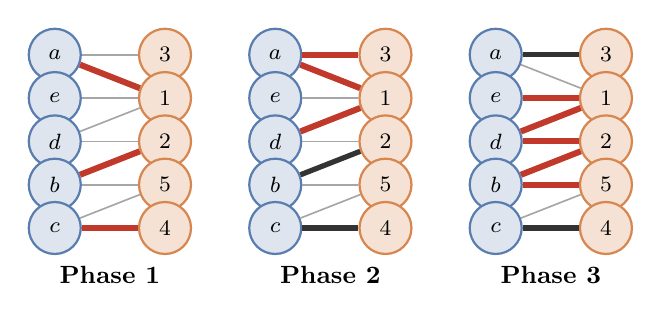
\begin{tikzpicture}[scale=0.5]
  \begin{scope}[shift={(0,0)}]
    \exnodes \exedges
    \draw[aug] (xa)--(y1); \draw[aug] (xb)--(y2); \draw[aug] (xc)--(y4);
    \node[font=\small\bfseries] at (1.4,-3.4) {Phase 1};
  \end{scope}
  \begin{scope}[shift={(5.6,0)}]
    \exnodes \exedges
    \draw[mat] (xb)--(y2); \draw[mat] (xc)--(y4);
    \draw[aug] (xd)--(y1); \draw[aug] (xa)--(y1); \draw[aug] (xa)--(y3);
    \node[font=\small\bfseries] at (1.4,-3.4) {Phase 2};
  \end{scope}
  \begin{scope}[shift={(11.2,0)}]
    \exnodes \exedges
    \draw[mat] (xa)--(y3); \draw[mat] (xc)--(y4);
    \draw[aug] (xe)--(y1); \draw[aug] (xd)--(y1); \draw[aug] (xd)--(y2);
    \draw[aug] (xb)--(y2); \draw[aug] (xb)--(y5);
    \node[font=\small\bfseries] at (1.4,-3.4) {Phase 3};
  \end{scope}
\end{tikzpicture}\\[1mm]
\small
\begin{tabular}{lccc}
\toprule
 & \textbf{Phase 1} & \textbf{Phase 2} & \textbf{Phase 3}\\
\midrule
Shortest augmenting length $\ell$ & 1 & 3 & 5\\
Levels of $\widetilde G$ & $L_0,L_1$ & $L_0..L_3$ & $L_0..L_5$\\
Paths found by Algorithm B & 3 & 1 & 1\\
$|M|$ & $0\to3$ & $3\to4$ & $4\to5$\\
\bottomrule
\end{tabular}
\end{center}
{\small\alert{As proved:} $\ell$ strictly increases ($1<3<5$); phases: $3\le2\lfloor\sqrt5\rfloor+2$.}
\end{frame}


\begin{frame}{Backup: proof of Theorem 2}
\begin{block}{Theorem 2}
Let $P$ be a shortest augmenting path for $M$ and $P'$ an augmenting path for $M\oplus P$. Then $\ |P'|\ \ge\ |P|+|P\cap P'|.$
\end{block}
\begin{plain}[In plain words]
Flipping a shortest path can only push the remaining augmenting paths \emph{further away}, never closer. If $P'$ reuses edges of $P$, it is even longer.
\end{plain}
\small\textbf{Proof.}
\begin{enumerate}\setlength\itemsep{0pt}
  \item $N=M\oplus P\oplus P'$ is a matching with $|N|=|M|+2$.
  \item Theorem 1: $M\oplus N=P\oplus P'$ contains two disjoint augmenting paths $P_1,P_2$ for $M$, each of length $\ge|P|$ ($P$ is shortest).
  \item So $|P\oplus P'|\ge2|P|$. But $|P\oplus P'|=|P|+|P'|-2|P\cap P'|$.
  \item Hence $|P'|\ge|P|+2|P\cap P'|\ \ge\ |P|+|P\cap P'|$. \hfill$\square$
\end{enumerate}
\end{frame}

\begin{frame}{Backup: proof of Corollary 4}

\textbf{Claim.} If $|P_i|=|P_j|$ then $P_i,P_j$ are vertex-disjoint.\\[2mm]
\textbf{Proof.} Suppose not. By Corollary 3 all lengths between $i$ and $j$ are equal. Pick a non-disjoint pair $P_k,P_l$ with $l-k$ \emph{minimal}; then every $P_m$ with $k<m<l$ is disjoint from both.
\begin{itemize}\setlength\itemsep{3pt}
  \item The flips of the $P_m$ do not touch $P_l$, so $P_l$ is still augmenting for $M_{k+1}=M_k\oplus P_k$.
  \item Theorem 2 with $|P_l|=|P_k|$: $P_k\cap P_l=\emptyset$ (no common edge).
  \item Suppose they share a vertex $v$. In $M_{k+1}$, $v$ is matched by an edge $e$ of $P_k$. $v$ is not an endpoint of $P_l$ (those are free), so $P_l$ passes through $v$ using its matching edge, which is $e$: a common edge. Contradiction. $\square$
\end{itemize}
\vspace{2mm}
\textbf{Why the exact count in Theorem 3.} Before $|M|=r$: lengths are odd numbers $\le2\lfloor\sqrt s\rfloor+1$, at most $\lfloor\sqrt s\rfloor+1$ of them. After: $\le s-r\le\lceil\sqrt s\rceil$ augmentations. Sum $\le2\lfloor\sqrt s\rfloor+2$.
\end{frame}

\end{document}
